%!TEX root = ../../thesis.tex
\subsection{Preliminaries on Lie groups}
Throughout this work, we will explore Lie group theory. We introduce the following notations: the Lie group of rigid-body transformation on $\R^3$ is denoted by $\SE{3}$, whereas the group of homogeneous rotation is denoted by $\SO{3}$. The tangent space at the identity of the group is called the Lie algebra, and it can be used to describe the evolution of the Lie group. The Lie algebra of $\SE{3}$ and $\SO{3}$ are denoted by $\seg{3}$ and $\sog{3}$, respectively. Lastly, the cross operator (i.e., "$\times$") and hat operator (i.e., "$\wedge$") are used to transform a column vector of $\R^3$ or $\R^6$ into an element of the Lie algebra $\sog{3}$ or $\seg{3}$, respectively.
%
\begin{figure}[!t]
  \vspace{-0.6mm}
  \centering
   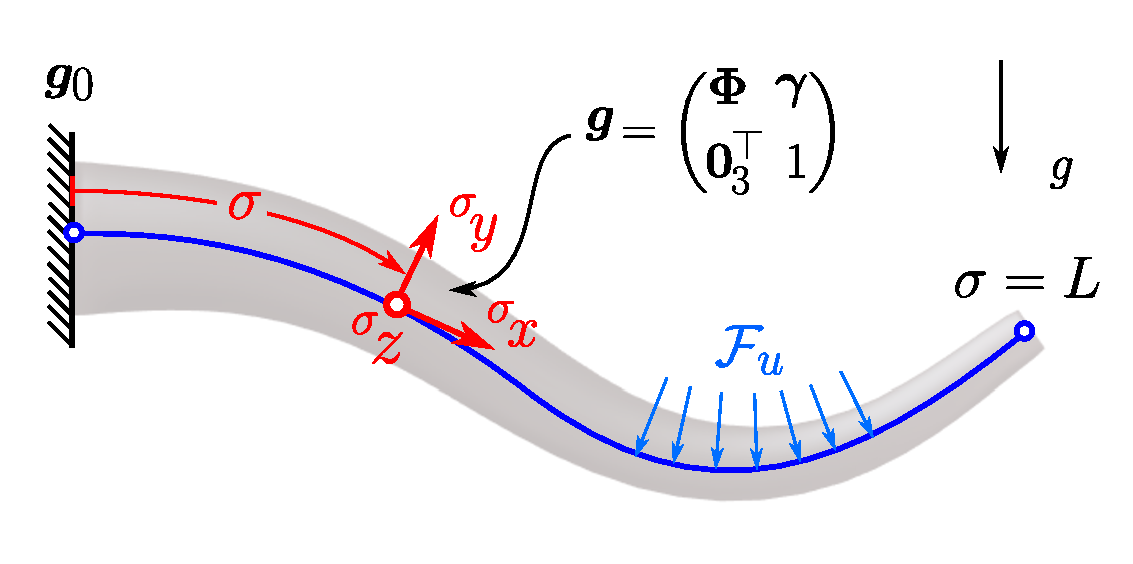
\includegraphics[width = 0.65\textwidth]{3_chapters/3_chapter/img/system.pdf}
  \caption{Schematic representation of a soft robot manipulator inspired by the tentacle of an octopus. The soft robot is model as a Cosserat beam with distributed actuation $\mathcal{F}_u$. \label{fig:example1}}
  \vspace{-0.1cm}
\end{figure}
%
\subsection{Cosserat beam theory}
In Cosserat theory, slender deformable solids are modeled as elastic strings subjected to geometric finite-strain theory. Drawing the analogy to soft robotics, we model the soft robot as a one-dimensional spatial curve passing through the geometric center of the soft robot (see Figure 1). Given its spatial-temporal nature, we introduce a temporal variable $t \in [0,\,T]$ with finite horizon time $T$, and a spatial variable $\sigma \in [0,\,L]$ with $L$ the undeformed length of the soft robot. For convenience, we denote $\Ts = [0,\,T]$ and $\Xs = [0,\,L]$. For each point on the backbone, we introduce a (mobile) coordinate frame. The homogeneous rotation related to these coordinate frames is given by the rotation matrix $\mat{\Phi}: \Xs \times \Ts \mapsto  \SO{3}$, and their origin by the position vector $\vec{\gamma}: \Xs \times \Ts \mapsto \R^3$.

Following the geometric approach \cite{Simo1986,Boyer2010,Boyer2021,Renda2018,Renda2020}, we may equivalently represent each coordinate frames that are rigidly attached to the continuous backbone of the soft robot by a parameterized space curve in $\SE{3}$:
%
\begin{equation}
\mat{g}(\sigma,t) = \begin{pmatrix} \mat{\Phi}(\sigma,t) & \mat{\gamma}(\sigma,t) \\ \vec{0}_3^\top & 1 \end{pmatrix} \in \SE{3}.
\end{equation}
%
Now, an expression for the strain field $\vec{\xi}$ and velocity field $\vec{\eta}$ anywhere on the Cosserat beam can be found by exploring the differential geometry of the curve. To do so, we must introduce some smoothness criteria:
%
\begin{asm}
\label{assum:1}
All control inputs, i.e., a distributed control wrench acting on the system, are considered to be sufficiently smooth for any instance $t \in \Ts$ and $\sigma \in \Xs$ such that the resulting parametrized backbone $\mat{g}(\sigma,t) \in \SE{3}$ is everywhere differentiable.
\end{asm}

\subsection{Local strain and velocity}
Following the works \cite{Renda2018,Renda2020,Boyer2021}, let $\vec{\Gamma} = (\kappa_1,\, \kappa_2, \kappa_3)^\top$ and $\vec{U} = (\nu_1,\, \nu_2,\, \nu_3)^\top$ be the torsion-curvature and elongation-shear strain vector, respectively. Then, an expression for strain field $\vec{\xi}(\sigma,t)$ is obtained through spatial differentiation of $\mat{g}$:
%
\begin{equation}
\hat{\vec{\xi}} := \mat{g}\inv \frac{\p \mat{g}}{\p \sigma} = \begin{pmatrix} \vec{\Gamma}^\times & \vec{U} \\[0.5em] \vec{0}_3^\top & 0 \end{pmatrix} \;\; \Longrightarrow \;\; \vec{\xi} := \begin{pmatrix} \vec{\Gamma} \\ \vec{U} \end{pmatrix}.
\label{eq:xi}
\end{equation}
%
Similarly, let $\vec{\Omega} = (\omega_1, \omega_2, \omega_3)^\top$ and $\vec{V} = (v_1,\,v_2,\, v_3)^\top$ be the angular and linear velocity vector, respectively. Then, an expression for velocity field $\vec{\eta}(\sigma,t)$ is obtained through time differentiation of $\vec{g}$:
%
\begin{equation}
\hat{\vec{\eta}} := \mat{g}\inv \frac{\p \mat{g}}{\p t} = \begin{pmatrix} \vec{\Omega}^\times & \vec{V} \\[0.5em] \vec{0}_3^\top & 0 \end{pmatrix} \;\; \Longrightarrow \;\; \vec{\eta} := \begin{pmatrix} \vec{\Omega} \\ \vec{V} \end{pmatrix}.
\end{equation}
%
Since we assume the $\mat{g}$ to be everywhere differentiable, we can derive a PDE for the continuous forward kinematics of the soft robot \cite{Boyer2021,Renda2020}:
%
\begin{equation}
\dfrac{\p \vec{\eta}}{\p \sigma} = -\textbf{ad}_{\vec{\xi}} \vec{\eta} + \dot{\vec{\xi}},
\label{eq:pde_kin}
\end{equation}
%
where $\ad_{(\cdot)}$ denotes the adjoint action on the Lie algebra (full derivation in Appendix A). Drawing an analogy to rigid robotics, the expression in \eqref{eq:pde_kin} may be seen as the forward velocity kinematics for a serial chain robot manipulator with infinitely many links.

%%%%%%%%%%%%%%%%%%%%%%%%%%%%%%%%%%%%%%%%%%%%%%%%%%
\subsection{Finite-dimensional reduction}
Similar to finite element methods, we wish to find a finite-dimensional approximation of the strain field $\vec{\xi}(\sigma,t)$ for all points on the material domain $\Xs$. To do so, we assume the following:
%
\begin{asm}
\vspace{1mm}
Assuming the strain field has a separable spatio-temporal nature, any entry of the strain vector field $\vec{\xi} = \left( \xi_1, \xi_2, ..., \xi_6 \right)^\top$ can be written as an infinite expansion of the following form:
%
\begin{equation}
\xi_i(\sigma,t) = \sum_{n=1}^\infty \theta_{n}(\sigma)q_{i,n}(t) + \xi^\circ_{i}(\sigma) \quad i\in\{1,\hdots,6\},
\label{eq:infinite_expans}
\end{equation}
%
where $\{\theta_{n}\}^\infty_{n=1}$ is the set of (orthogonal) basis functions $\theta_{n}: \Xs \to \R$ together with modal coefficients $q_{i,n}: \Ts \to \R$, and an intrinsic time-invariant strain $\xi^\circ_{i}: \Xs \to \R$. The basis functions $\theta_{n}(\cdot)$ and the modal coefficients $q_n(\cdot)$ are both smooth functions.
\end{asm}

\begin{asm}
Given infinite expansion \eqref{eq:infinite_expans}, the $k$-th order truncation for any entry of the strain field, defined as
%
\begin{equation}
[\xi_i]_k(\sigma,t) := \sum_{n=1}^k \theta_n(\sigma)q_{i,n}(t) + \xi^\circ_{i}(\sigma) \quad i\in\{1,\hdots,6\},
\end{equation}
%
converges uniformly on $\Xs$ and $\Ts$ as the index $k \to \infty$. Moreover, we assume that uniform convergence holds for its partial derivatives $\tfrac{\p}{\p t} [\vec{\xi}]_k$ and $\tfrac{\p}{\p \sigma} [\vec{\xi}]_k$.
\end{asm}

\noindent Accordingly, we can rewrite the $k$-th order truncation of the complete strain field as a linear matrix operation as follows
%
\begin{multline}
[\vec{\xi}]_k  = \left(\vec{I}_6  \otimes \begin{bmatrix} \theta_1 & \hdots & \theta_k \end{bmatrix} \right) \vec{q} + \vec{\xi}^\circ,  \\[0.5em]
 =
\begingroup % keep the change local
\setlength\arraycolsep{2.5pt}
\underbrace{\begin{pmatrix}
\theta_1 & \hdots & \theta_k & \hdots & 0 & \cdots&  0 \\
\vdots & \ddots & \vdots & \ddots & \vdots & \vdots & \vdots \\
0 & \cdots&  0 & \hdots & \theta_1 & \hdots & \theta_k\end{pmatrix}}_{{\mat{\Theta}(\sigma)}}
\endgroup
\underbrace{\begin{pmatrix} q_{1,1} \\ \vdots \\ q_{6,k}\end{pmatrix}}_{\vec{q}(t)} + \vec{\xi}^\circ,
\label{eq:trunc_2}
%\vspace{-4mm}
\end{multline}
%
where $\mat{\Theta} \in \R^{6 \times 6k}$ is a sparse matrix-valued function whose columns are mutually orthonormal, the operator $\otimes$ denotes the Kronecker product, and the vector $\vec{q} \in \R^{6k}$ the collection of all time-variant modal coefficients related to the columns of $\mat{\Theta}$. Although a wide variety of bases are possible \cite{Boyer2021,Santina2020}, we have chosen a modified Legendre polynomial set:
%
\begin{equation}
\theta_n(\sigma) = \frac{2}{2^{n}(n-1)!} \frac{d^{n-1}}{d\sigma^{n-1}}\left[\left( \tfrac{2\sigma}{L_0}-1 \right)^2 -1 \right]^{n-1}
\end{equation}
%
with $n \in \Z^+$ the polynomial degree. Please note now that the inner product between elements of the set of modified Legendre functionals $\{\theta_n\}_{n = 1}^k$ satisfies $\inner{\theta_i}{\theta_j}_{\Xs} := \int_\Xs{\theta_i}{\theta_j} d\sigma = 0$ for $i \neq j$, and $1$ otherwise. An alternative option could be constructing the set of basis functions through the so-called '\textit{snapshot decomposition method}' using FEM-driven data \cite{Astrid2008,Duriez2013,Largilliere2015}.

\subsection{Finite-dimensional kinematics}
Given the finite-dimensional truncation in \eqref{eq:trunc_2}, we can now find an expression for the finite-dimensional forward kinematics in terms of the generalized coordinates $\vec{q}$ and its velocities components $\dot{\vec{q}}$.

First, let us regard the configuration of the soft robot $\mat{g} \in \SE{3}$. Recall that the spatial evolution of the curve is described by $\p \mat{g}/\p\sigma = \mat{g} \vec{\xi}^\wedge$, see Eq. \eqref{eq:xi}. Given the initial condition $\mat{g}(0,\cdot) = \mat{g}_0$, an approximation of the continuously deformable soft robot can be obtained by partial integration over the spatial domain:
%
\begin{equation}
[\mat{g}]_k(\sigma,\vec{q}) = \mat{g}_0 \exp\left[\int_0^\sigma [\hat{\vec{\xi}}]_k(s,\vec{q}) \; ds \right].
\end{equation}
%
Please note that this nothing more than the reconstruction of the curve by integration of its tangent space along its spatial parameter $\sigma$. Next, lets regard the velocity kinematics $\vec{\eta}(\sigma,t)$ for any point $\sigma$ on the backbone curve. Using the differential property of the adjoint action $\mat{\ad}_{\vec{\xi}} = -\p /\p \sigma [\Ad_{g^{-1}}] \Ad_{g}$ \cite{Murray1994}, we can rewrite the continuous forward kinematics in \eqref{eq:pde_kin} as
%
\begin{equation}
\frac{\p \vec{\eta}}{\p \sigma } = \frac{\p }{\p \sigma }\left(\mat{\Ad}_{\mat{g}^{-1}}\right) \mat{\Ad}_{\mat{g}} \vec{\eta} + \dot{\vec{\xi}}. \label{eq:eta_adg}
\end{equation}
%
Now, given the initial condition $\vec{\eta}(0,t) = \vec{0}_6$ and the approximations $[\vec{\xi}]_k$ and $[\mat{g}]_k$, we can find an approximation to the velocity twist $\vec{\eta}$ by partial integration over space:
%
\begin{equation}
[\vec{\eta}]_k(\sigma,\vec{q},\dot{\vec{q}}) = \Ad_{[\mat{g}]_k}\inv \int_0^\sigma \Ad_{[\mat{g}]_k} \mat{\Theta} \; ds \,\dot{\vec{q}} := [\mat{J}]_k\, \dot{\vec{q}}, \label{eq:eta_analytic}
\end{equation}
%
which naturally gives rise to the geometric Jacobian $[\mat{J}]_k \in \R^{6\times 6k}$. The geometric Jacobian plays an important role in obtaining the Lagrangian form of the reduced-order dynamic model. Finally, to express the acceleration twist, we take the time-derivative of \eqref{eq:eta_analytic} leading to
%
\begin{align}{}
[\dot{\vec{\eta}}]_k & = [\mat{J}]_k\ddot{\vec{q}} + \dot{[\mat{J}]}_k\dot{\vec{q}}, \notag \\
& = [\mat{J}]_k\ddot{\vec{q}} + \Ad_{[\mat{g}]_k}\inv \int_0^\sigma \Ad_{[\mat{g}]_k} \ad_{[\vec{\eta}]_k} \mat{\Theta} \; ds \,\dot{q} \label{eq:deta_analytic},
\end{align}
%
which gives rise to the analytic expression of the time-derivative of the geometric Jacobian $\dot{[\mat{J}]}_k$ (\highlight{see Appendix B for the derivation}).

\subsection{Finite-dimensional dynamics}
Here, we detail the dynamics of the Cosserat beam. A majority of the dynamic framework presented here is adopted from \cite{Boyer2021}; yet we introduce some modification to allow a pH-structure.
First, let us consider an infinitesimal slice of continuum body that is perpendicular to the backbone curve. The kinetic momenta of this infinitesimal slice is then given by $\vec{\mu}(\sigma,t) = \mat{\Mt} \vec{\eta}(\sigma,t)$ in which $\Mt \in \cose{3} \times \seg{3} \cong \R^{6\times 6}$ denotes the symmetric inertia tensor.
%
\begin{rmk}
For some soft robots, the inertia tensor $\mat{\Mt}$ may have an explicit dependency on space or time (or both). Nevertheless, for sake of simplicity, we limit ourselves to a diagonal invariant inertia tensor $\mat{\Mt} = \diag{\rho \mat{I}_3, \rho \mat{\mathcal{J}}}$ with line-density $\rho > 0$ and the second moment of area $\mat{\mathcal{J}} \in \coso{3} \times \sog{3} \cong \R^{3\times 3}$.
\end{rmk}
%
\noindent Using the expression of the kinetic momenta $\vec{\mu}$ of the infinitesimal body, we can write the equation of motion for a particular slice at $\sigma$ using the Newton-Euler equations:
%
\begin{equation}
\frac{\p }{\p t} (\Ad_{g}^{-\top} \vec{\mu}) = \Ad_{g}^{-\top}\Ft,\label{eq:newton_euler}
\end{equation}
%
% where again $\Ad_{(\cdot)}$ stands for the adjoint action, and $\vec{\Ft} = \vec{\Ft}_c  + \vec{\Ft}_u - \vec{\Ft}_g - \vec{\Ft}_e$ the resultant wrench that is composed of the constraint wrench $\vec{\Ft}_c$, the input wrench $\vec{\F}_u$, and the potential wrenches due to gravity and visco-elasticity, $\vec{\Ft}_g$ and $\vec{\Ft}_e$, respectively. Further evaluation of \eqref{eq:newton_euler} leads to
